\documentclass{article}
\usepackage{oeNIKstyle}
\author{Kővári Bence}
\neptunCode{IFWY0R}
\courseName{Adatbázis és big data technológiák}
\documentumTypeName{Feladat dokumentáció}

\title{Csatlakozási lehetőségek tesztelése}



\begin{document}
\section{Csatlakozási lehetőségek tesztelése}
\subsection{Oracle Cloud Services Oracle adatbázis}
Szeretnék az Oracle Cloud Services (OCI)-n belül létrehozni egy Oracle adatbázist, és azt csatlakoztatni a vizualizációs eszközhöz. Ennek érdekében regisztráltam egy trial accountot, és létrehoztam egy Oracle Database Instance-t. Az adatbázis egy Standard Edition 12.2-es verziójú. Ezt követően a új kapcsolatot hoztam létre a csatlakozás érdekében:
\begin{figure}[h!]
	\centering
	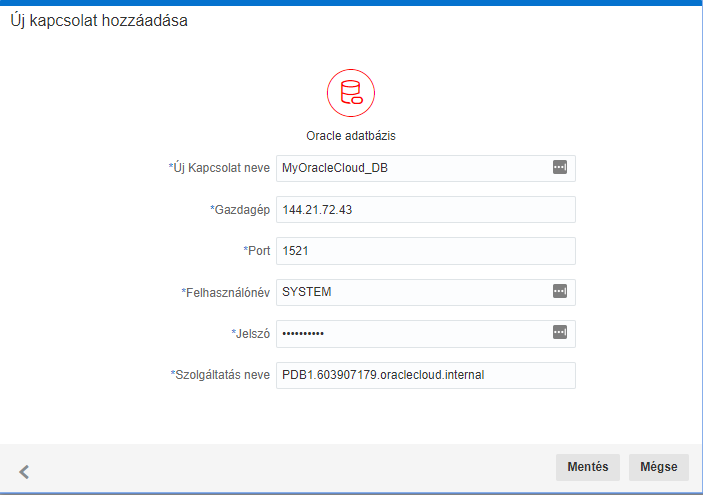
\includegraphics[width=0.9\linewidth,height=0.45\linewidth]{add_connection_oracleclouddb}
	\caption{Új Oracle Cloud-beli Oracle kapcsolat hozzáadása}
	\label{fig:addconnectionoracleclouddb}
\end{figure}
Az adatbázishoz hozzákapcsolódtam SQL Developer klienst használva, és létrehoztam két teszttáblát \textit{AIRLINE} és \textit{AIRPORT} névvel, melyeket tesztadatokkal feltöltöttem. Ezt követően szerettem volna ezeket a táblákat adatforrásként használni, de amikor hozzá kívántam adni, nem jelentek meg az elérhető táblák között. Az elérhető táblák közt szerepelt \textit{HELP} nevű tábla, melyet próbaként töröltem az adatbázisból, de hiába kattintottam az adatok frissítésére, a tábla továbbra is ott maradt. 
\newpage\begin{figure}[h!]
	\centering
	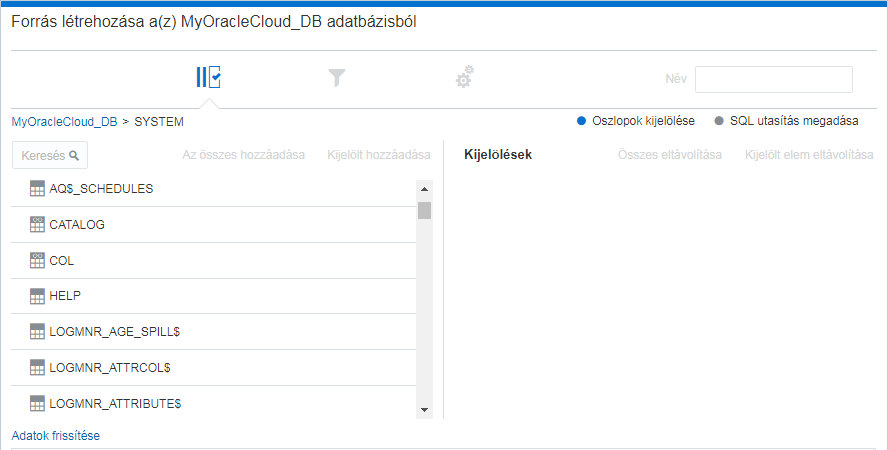
\includegraphics[width=0.7\linewidth]{add_datasource_fromdb}
	\caption{Elérhető táblák listája}
	\label{fig:adddatasourcefromdb}
\end{figure}
A \ref{fig:adddatasourcefromdb}. ábrán látható az elérhető táblák listája. A listában a \textit{HELP} tábla a törlést követően frissítés ellenére is megjelenik, valamint a létrehozott teszt táblák továbbra sem elérhetőek. Összefoglalva tehát a SYSTEM user alatt csak konstant táblákat láttam, melyek létrehozhás/törlés műveletekre nem reagáltak, frissítés ellenében sem. Megpróbáltam azt is, hogy újra létrehozom a kapcsolatot, de ugyanazt a konstans listát látom a SYSTEM user alatt a táblák tekintetében azesetben is.
\subsection{Amazon Web Services Oracle adatbázis}
Ezen alfejezet célja az Oracle adatbázishoz való csatlakozás tesztelése Amazon Web Services-en létrehozott Oracle adatbázis segítségével.. A kivitelezéshez létrehoztam az AWS RDS szolgáltatásával egy Oracle adatbázist futtató instancet. Az adatbázis Oracle Standard Edition 11.2.0.4.v16 verziójú, és publikus végponttal rendelkezik, helyileg Frankfurt régióban.

\begin{figure}[h!]
	\centering
	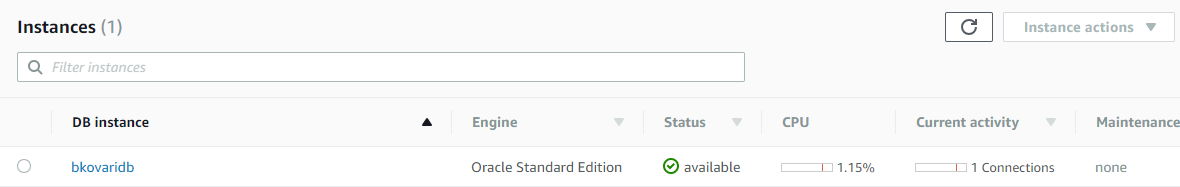
\includegraphics[width=1\linewidth,height=0.2\linewidth]{oracle_db}
	\caption{Oracle Standard Edition instance}
	\label{fig:oracledb}
\end{figure}
Az adatbázishoz először SQL Developer klienst használva csatlakoztam, hogy ellenőrizzem az elérhetőséget. Csatlakozáskor a megfelelő SID-t használva (ORCL) léptem be az adatbázisba. Mivel a Visualisation Tool csatlakozáskor nem SID-t használ, ezért egy \textit{show parameters service name} lekérdezést futtattva lekérdeztem az adatbázisom Service Name-t, mely ORCL\_A nevet viseli. \\ Ezt követően megkíséreltem az adatforrást hozzáadni a Visualization Tool-ban "Új kapcsolatot" létrehozásával, Oracle adatbázist kiválasztva.
\begin{figure}[h!]
	\centering
	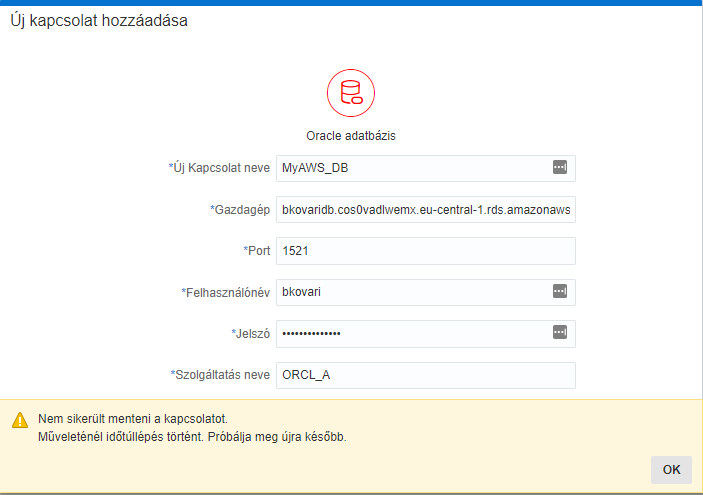
\includegraphics[width=0.9\linewidth,height=0.45\linewidth]{add_connection_aws}
	\caption{Új AWS-beli Oracle kapcsolat hozzáadása}
	\label{fig:addconnectionaws}
\end{figure}
A csatlakozáshoz megadtam a megfelelő adatokat, viszont időtúllépés hiányában a kapcsolat nem jött létre. SQL Developerrel SID használata helyett ORCL\_A Service Name segítségével a csatlakozás viszont sikeres volt. Megpróbáltam még Oracle Enterprise Edition 12.1.0.2.v12 verziójú adatbázissal is, de ugyanezt tapasztaltam. Konkrét információt erre vonatkozólag nem találtam, viszont ebből arra következtetek, hogy csak az Oracle Cloudban létrehozott Oracle adatbázissal képes az a Visualisation Tool kommunikálni.

\end{document}